\section{Introduction}
\label{sec:dbb:intro}

As discussed in Chapter~\ref{ch:pastwork}, alkaline batteries are the mainstay of the primary battery market. The LR6 form factor {\ce{Zn-MnO_2}} battery, or the ``alkaline" AA battery accounted for \$1.8 billion of worldwide battery sales in 2013 alone.~\cite{highbeam,ibisworld} The simply manufactured bobbin cell design, reproduced below from Fig.~\ref{fig:aaschem}, has contributed to the cell's popularity in the last 50 years.~\cite{karl_patent}

\begin{figure}[htb]
  \centering
    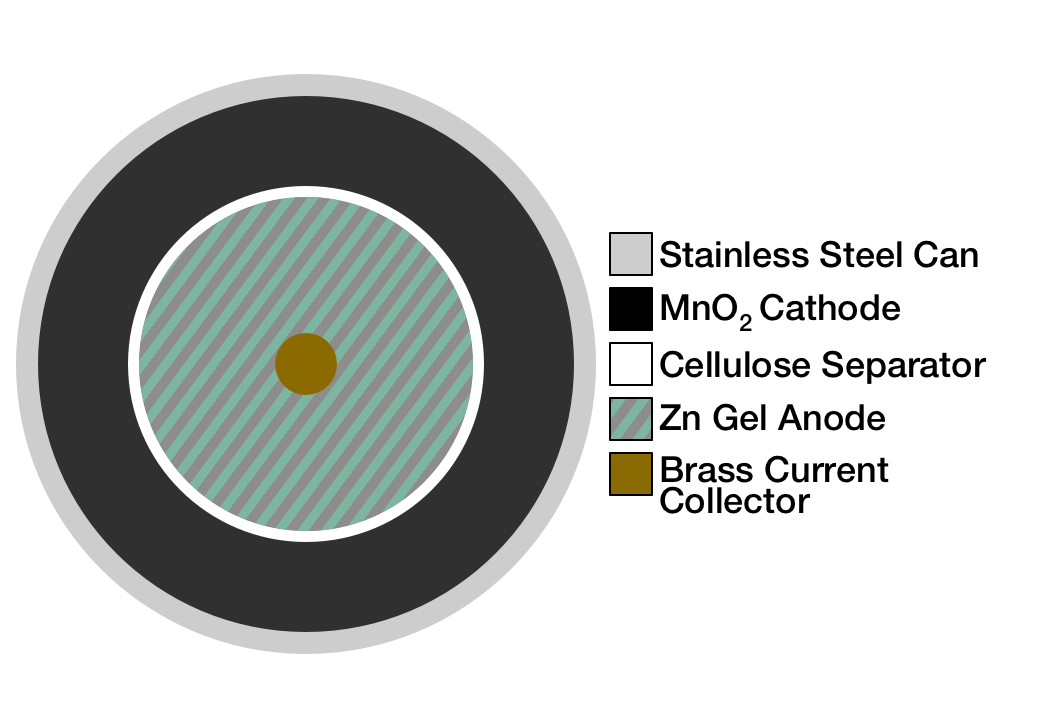
\includegraphics[width=0.80\textwidth]{ch3-dbb/Images/aaschem.png}
    \repeatcaption{fig:aaschem}{Schematic of construction of a alkaline AA battery. Components are labeled according to the legend.}
\end{figure}

Electrical testing is the accepted method of determining a battery's health, but mechanical testing of batteries has surfaced as a viable method for determining the material properties of a battery. Methods have probed the mechanical behavior of the separator, ~\cite{cannarella_ion,peabody_separator} the electrodes,~\cite{chen,du_cycling,han,park,striebel} and the entire cell.~\cite{cannarella_stress} The destructive nature of some of these methods makes them unfeasible for applications in which the cell must remain intact. Methods such as X-ray diffraction (XRD),~\cite{gallaway} X-ray microtomography,~\cite{haibel,Manke2007-yj,ebner} and acoustic emission sensing~\cite{etiemble,kalnaus,kircheva,rhodes} allow for non-destructive \textit{in situ} characterization of the microstructure, but both methods require specialized equipment and, with few exceptions, cannot be applied \textit{in operando}.

Recently there has been popular interest~\cite{youtube} in the tendency of an alkaline AA battery to bounce after being dropped on its end when discharged to full capacity, compared to a flat landing with minimal bounce when the battery is ``as-received". In this chapter, focuses on this bounce test and how it may provide information about a alkaline AA battery's state of charge and state of health. The coefficient of restitution (COR) of an alkaline AA battery is measured at various depths of discharge by dropping the battery in a controlled fashion and observing the subsequent bouncing, and the change in COR is then compared to spatially resolved energy-dispersive x-ray diffraction (EDXRD) that was performed \textit{in situ} on equivalent alkaline AA batteries. Our measurements show that this simple bounce test provides a considerable amount of information of the structure of the battery's Zn anode, rivaling the sensitivity of \textit{in situ} EDXRD in detection of ZnO formation. 

This chapter focuses on how non-destructive dynamic mechanical testing using the bounce test can relate properties of the bulk battery to properties of the individual components. By elucidating upon the nature of the relationship between COR and state of charge, it lays the foundation for \textit{in operando} dynamic mechanical testing, detailed in chapters~\ref{ch:bw} and~\ref{ch:alkbw}.
